\chapter{Part III(a) - Memory Hierarchy - Caches}
\textit{Memory is a fundamental component of computing systems, as its performance directly impacts the speed at which data can be accessed and processed, influencing overall system efficiency.} \\
\textbf{The balance we aim to achieve lies in optimizing speed to meet the demands of the CPU while maximizing memory capacity to satisfy our requirements.}
\section{Our Goal : Use Different Memories}
\textit{Instad of using a single memory, with fixed monolothitic caracteristics, we can use a hierarchy of memories, each with different characteristics.}
\begin{center}
    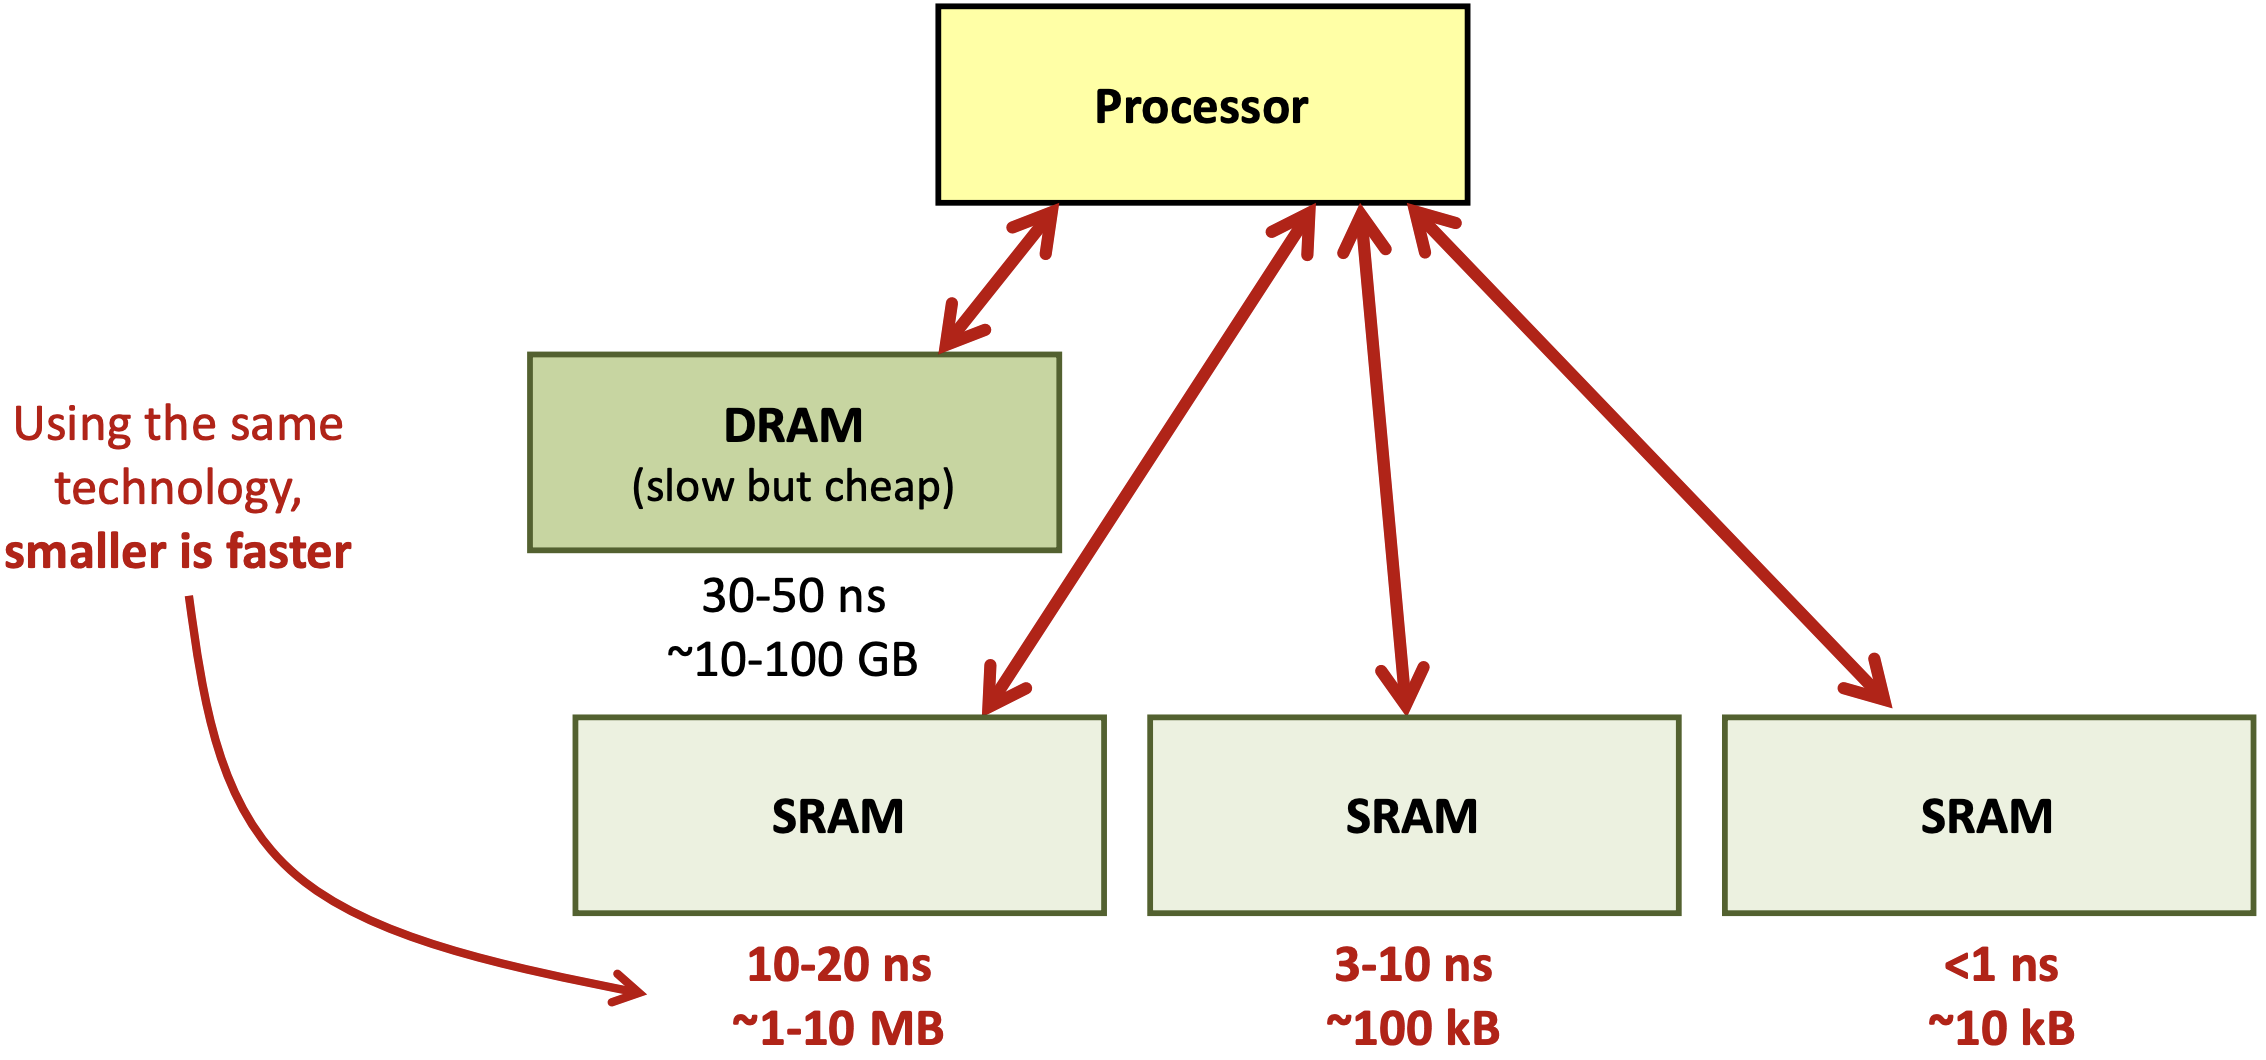
\includegraphics[width=0.65\textwidth]{chapters/chapter3a/images/hierarchy.png}
\end{center}
\begin{itemize}
    \item \textbf{DRAM (Dynamic Random Access Memory):}
    \begin{itemize}
        \item \textit{Characteristics:} DRAM is slow but cost-effective.
        \item \textit{Access Time:} Typically between 30 and 50 nanoseconds.
        \item \textit{Capacity:} Provides a large storage size, ranging from 10 GB to 100 GB.
    \end{itemize}
    
    \item \textbf{SRAM (Static Random Access Memory):}
    \begin{itemize}
        \item \textit{Characteristics:} SRAM is fast but expensive.
        \item \textit{Access Time:} Less than 1 nanosecond.
        \item \textit{Capacity:} Offers smaller storage sizes, around 10 KB.
    \end{itemize}
\end{itemize}

\textbf{Objective:} The goal is to leverage the advantages of both DRAM and SRAM to achieve an efficient memory system, combining the speed of SRAM with the cost-effectiveness and capacity of DRAM.

\begin{center}
    \textit{Can we get the best of both worlds?}
\end{center}


\subsection{What Memory ot Use?}
Efficient memory usage is crucial for ensuring high performance in iterative computations, as seen in the following example:
\begin{cc}
i = 0;
sum = 0;
while (i < 1024) {
    sum = sum + a[i];
    i = i + 1;
}
\end{cc}
\begin{itemize}
    \item \textbf{Instruction locality:} Instructions corresponding to lines 3-5 in the loop are read repeatedly. These should reside in fast memory (e.g., caches) to minimize latency.
    \item \textbf{Variable access:} Frequently accessed variables like \texttt{i} and \texttt{sum} should be stored in fast memory, such as registers or cache, to reduce access time.
    \item \textbf{Prefetching:} To improve performance, future instructions and array elements (e.g., \texttt{a[i+1]}, \texttt{a[i+2]}, etc.) can be loaded into memory in advance using techniques like hardware or software prefetching.
\end{itemize}

\subsection{Spatial and Temporal Locality}
Two important criteria for deciding on data placement in memory are:

\paragraph{Temporal Locality} This refers to data that has been \textbf{used recently} and thus has a high likelihood of being reused. Examples include:
\begin{itemize}
    \item \textbf{Code:} loops, functions, etc.
    \item \textbf{Data:} local variables and data structures.
\end{itemize}

\paragraph{Spatial Locality} This refers to data located \textbf{near other data currently in use}, which is likely to be accessed soon. Examples include:
\begin{itemize}
    \item \textbf{Code:} sequentially read instructions.
    \item \textbf{Data:} arrays and other contiguous structures.
\end{itemize}

\subsection{Placement Policy Design}

Our placement policy must satisfy two essential requirements:

\begin{itemize}
    \item \textbf{Invisible to the Programmer:}
    \begin{itemize}
        \item While it is possible to analyze data structures and program semantics to detect heavily used variables or arrays for placement decisions, this approach is only suitable in specific contexts (e.g., embedded systems).
        \item The goal is to alleviate the burden on programmers by introducing hardware mechanisms to manage placement transparently.
    \end{itemize}
    \item \textbf{Extremely Simple and Fast:}
    \begin{itemize}
        \item Placement decisions, when delegated to hardware, must be simple to ensure efficiency.
        \item The primary objective is to facilitate access to fast memory within nanoseconds or less, leaving little room for complex decision-making.
    \end{itemize}
\end{itemize}
\newpage
\section{Cache: The Idea}
Caching is a mechanism used to improve the performance of a computer system by storing frequently accessed data in a smaller, faster memory known as the cache. 
\begin{center}
    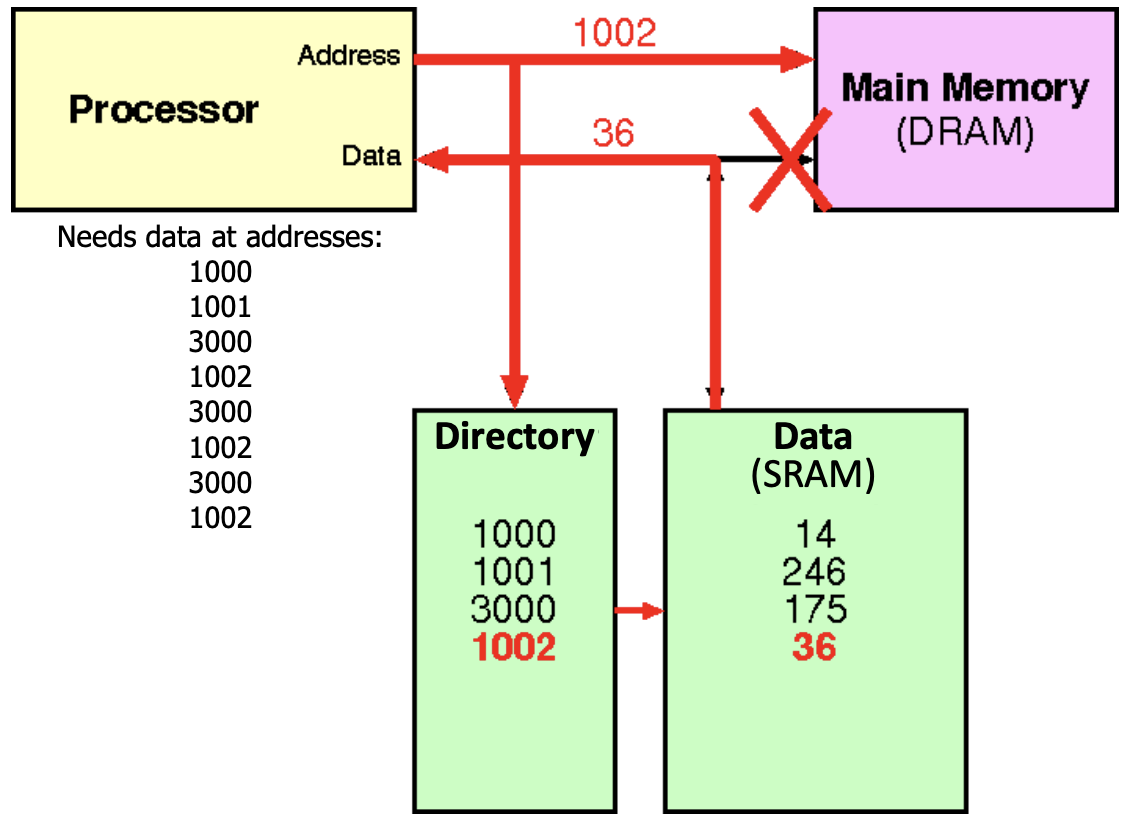
\includegraphics[width=0.45\textwidth]{chapters/chapter3a/images/cache.png}
\end{center}
\begin{itemize}
    \item[-] \textbf{Processor Request:} The processor requires data located at specific memory addresses, such as \texttt{1000}, \texttt{1001}, \texttt{3000}, and \texttt{1002}.
    \item[-] \textbf{Cache Directory and Data:} The cache maintains a directory that maps memory addresses to their corresponding data stored in the cache. For example, the data for address \texttt{1002} is located in the cache with a value of \texttt{36}.
    \item[-] \textbf{Cache Hit:} If the requested address exists in the cache directory (e.g., \texttt{1002}), the processor retrieves the data directly from the cache. This is referred to as a \textit{cache hit}.
    \item[-] \textbf{Cache Miss:} If the requested address is not found in the cache, the data is fetched from the main memory (DRAM), stored in the cache, and then delivered to the processor.
    \item[-] \textbf{Performance Benefit:} By prioritizing access to the cache (SRAM), which is faster than main memory (DRAM), the system reduces latency and improves overall performance.
\end{itemize}


\subsection{Cache Memory: Directory and Tags}
Cache memory is not just about speed but also about efficient management of data. Two critical components of a cache system are the \textbf{Directory} and \textbf{Tags}, which play a vital role in ensuring data consistency and fast access.
\begin{center}
    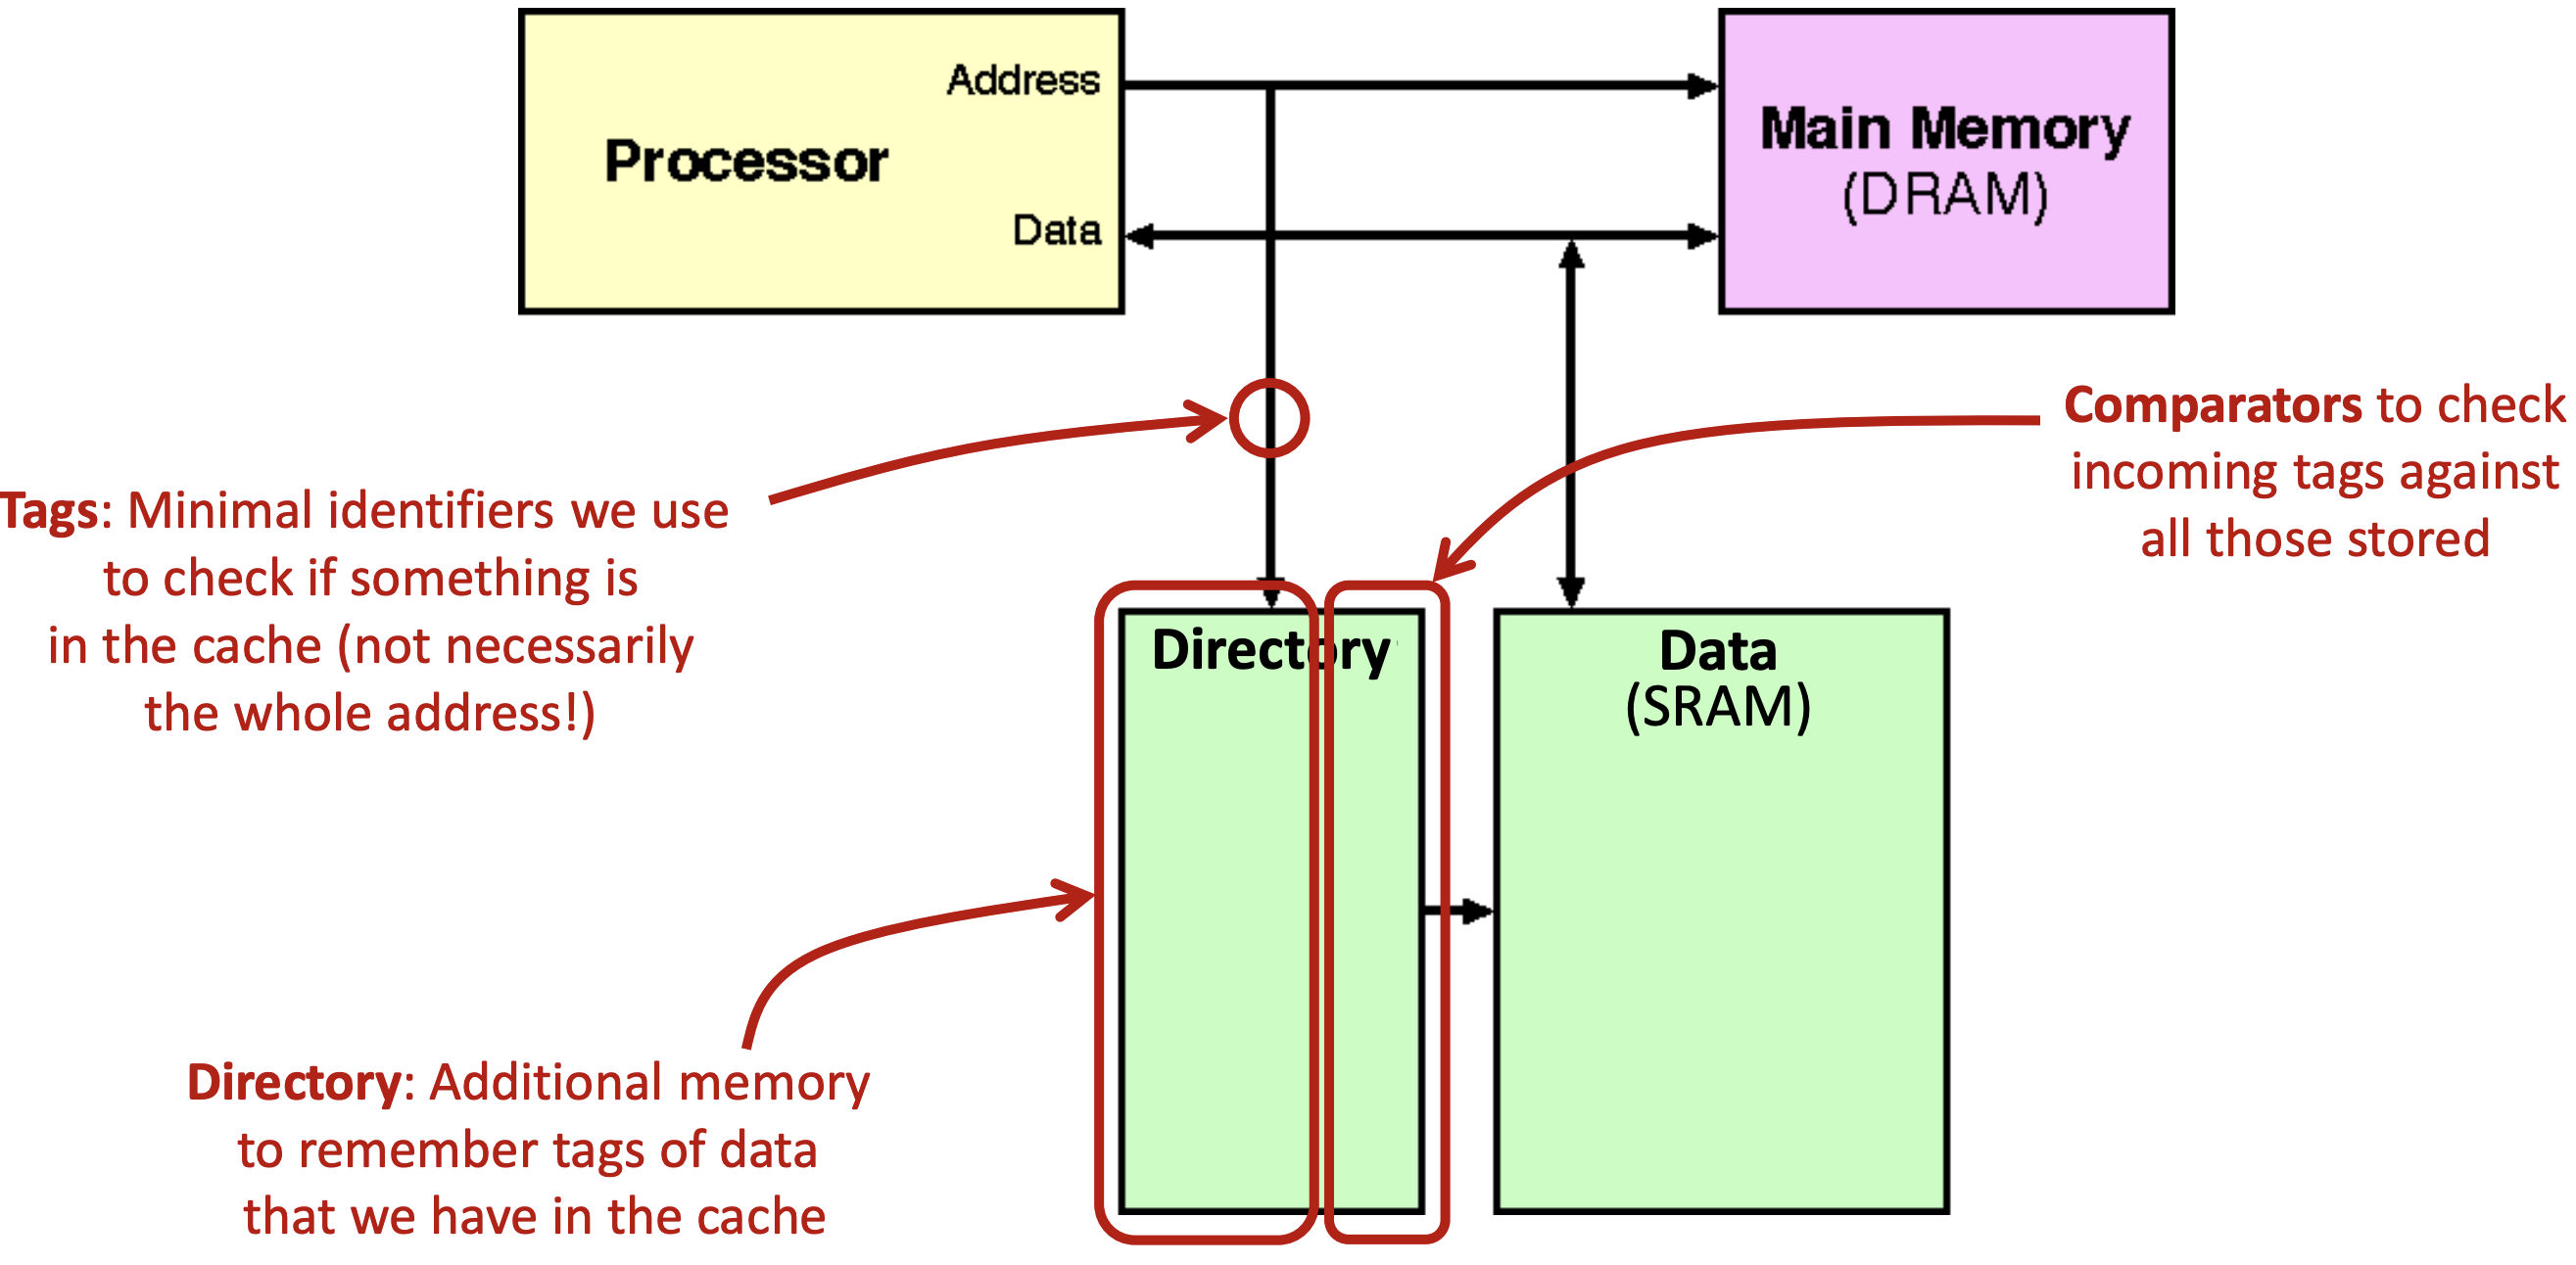
\includegraphics[width=0.65\textwidth]{chapters/chapter3a/images/cache2.png}
\end{center}
\begin{itemize}
    \item[-] \textbf{Tags:} Minimal identifiers used to determine if a specific data block is in the cache. These identifiers are typically smaller than the full memory address, optimizing comparison speed and storage requirements.
    \item[-] \textbf{Directory:} A dedicated memory structure that stores the tags of data currently present in the cache. This allows for efficient lookups and ensures the correct data is retrieved.
    \item[-] \textbf{Comparators:} Hardware elements that compare incoming tags against those stored in the directory. They enable quick validation of cache hits or misses.
\end{itemize}

\subsection{Cache Hits and Misses}
A \textbf{cache} is a form of storage that \textit{automatically} leverages the \textbf{locality of accesses} to improve performance. The concept has been widely adopted beyond processors, and examples include:

\begin{itemize}
    \item[-] Web browsers caching frequently accessed data.
    \item[-] Network routers caching routing information.
    \item[-] DNS servers caching frequent domain names.
    \item[-] Databases caching queries.
\end{itemize}

When the required data is found in the cache, it is called a \textbf{Hit}. Conversely, if the data is not found, it is termed a \textbf{Miss}.

The \textbf{Hit Rate} (or \textbf{Miss Rate}) is defined as the ratio of hits (or misses) to the total number of accesses.


\subsection{Fully-Associative Cache}

A fully-associative cache is a type of cache memory that allows any block of main memory to be stored in any cache line. 

\begin{center}
    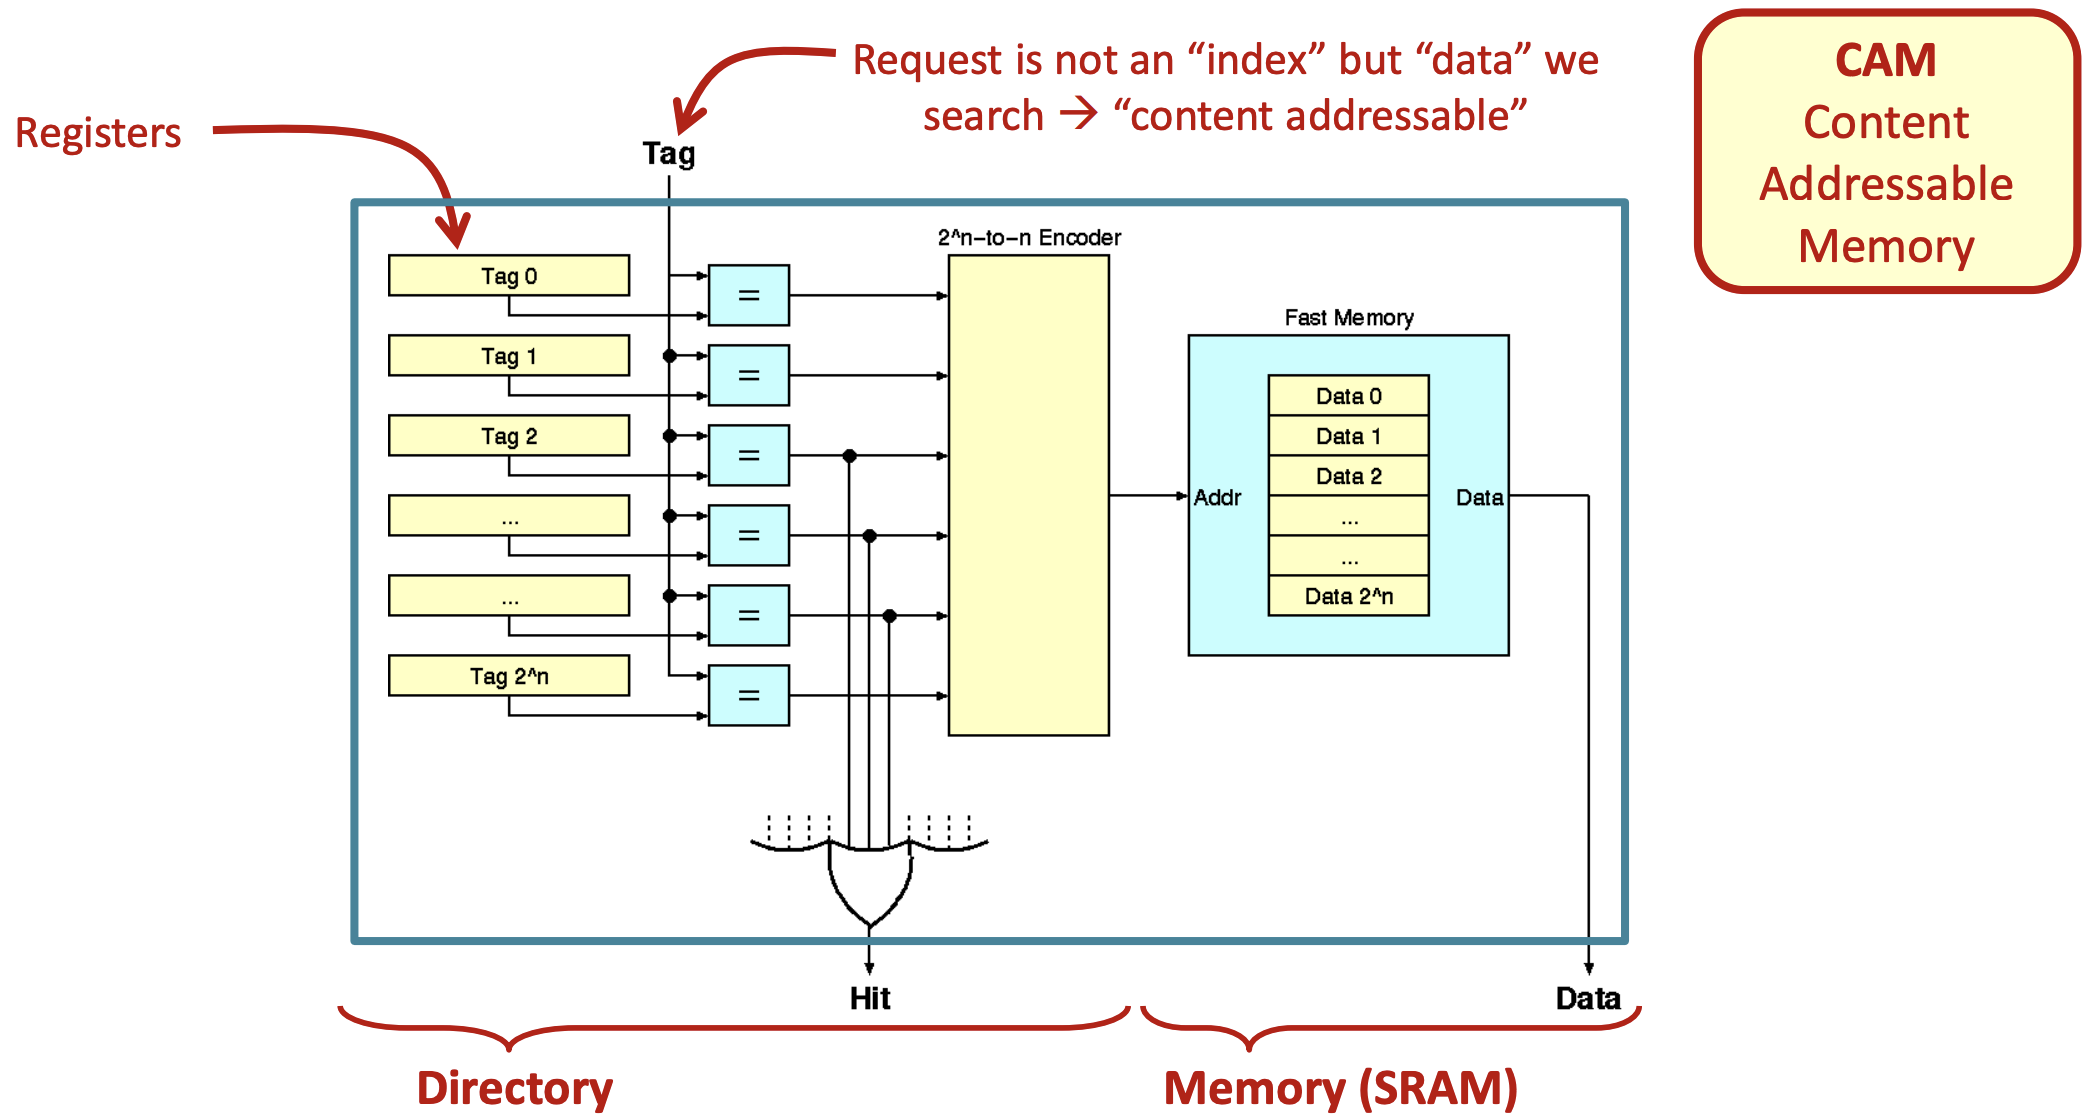
\includegraphics[width=0.75\textwidth]{chapters/chapter3a/images/cache3.png}
\end{center}
\subsubsection*{Key Components}
\begin{enumerate}
    \item \textbf{Directory (Tag Array):} Each entry in the tag array (referred to as "Tags") stores metadata about the cached blocks. Tags uniquely identify the memory block stored in each cache line.
    \item \textbf{Content Addressable Memory (CAM):} To find a specific block in the cache, the requested address is compared simultaneously with all stored tags. This parallel comparison is achieved using CAM, which enables \textit{content-based addressing}.
    \item \textbf{Comparison Logic:} The CAM outputs a signal indicating whether the requested tag matches any of the stored tags. This determines a \textit{hit} or \textit{miss}.
    \item \textbf{Fast Memory (SRAM):} This stores the actual data blocks associated with each tag. When a hit occurs, the data corresponding to the matched tag is retrieved from this memory.
    \item \textbf{Encoder:} If a match (hit) is found, the encoder selects the appropriate line from the data memory to access the requested data.
\end{enumerate}

\subsubsection*{How It Works}
\begin{enumerate}
    \item A memory access request is initiated with an address containing the desired data's \textit{tag}.
    \item The tag is compared in parallel against all tags stored in the directory using CAM.
    \item If a match is found, a \textit{hit} is signaled, and the corresponding data is retrieved from the fast memory using the encoder. If no match is found, a \textit{miss} occurs, and the block is fetched from main memory.
    \item The requested data is returned to the processor.
\end{enumerate}

\subsection{Fully-Associative Cache}

In a \textit{fully-associative cache}, any block of memory can be stored in any cache line. This flexibility removes the need for a specific mapping between memory blocks and cache lines, allowing for maximum utilization of cache space. 

\begin{center}
    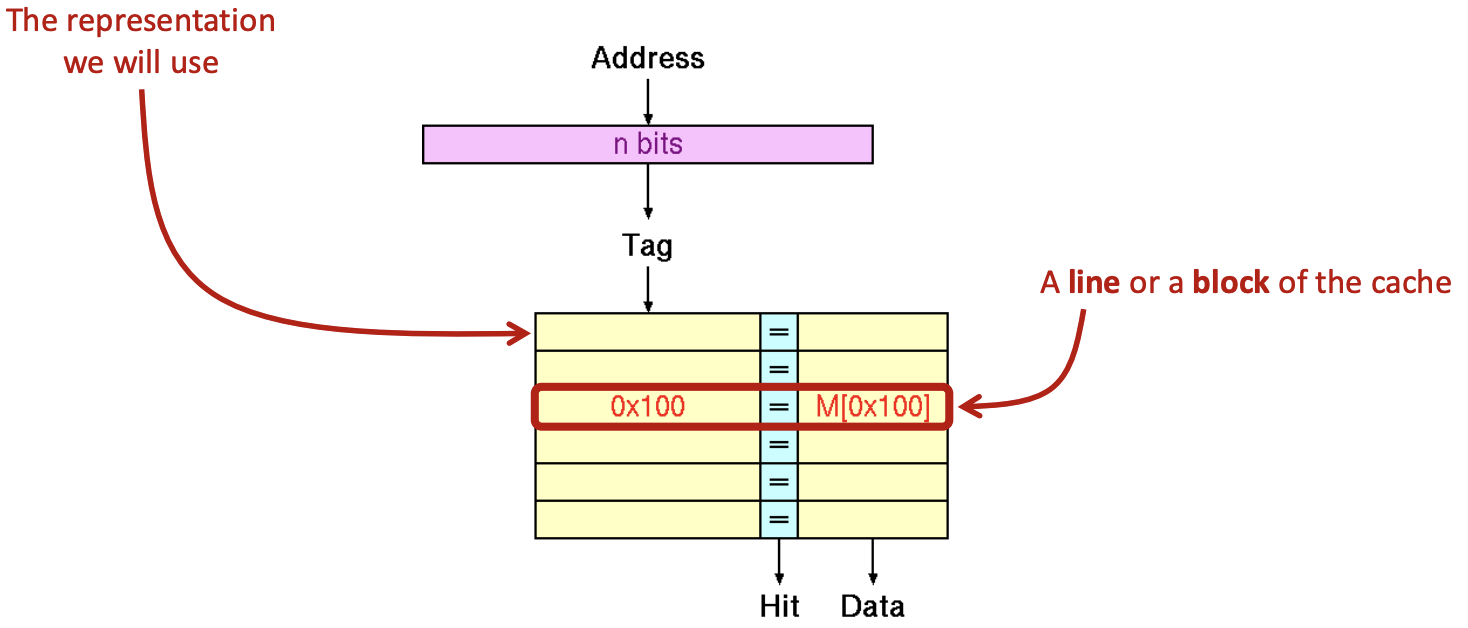
\includegraphics[width=0.65\textwidth]{chapters/chapter3a/images/cache4.png}
\end{center}
\begin{itemize}
    \item[-] \textbf{Address Representation:} The memory address is represented using $n$ bits. Each address can be divided into a \textit{tag} and an optional \textit{block offset} (if the cache stores data in blocks).
    \item[-] \textbf{Cache Lines:} Each line (or block) of the cache contains:
    \begin{enumerate}
        \item The \textit{tag} to identify the memory block stored in that line.
        \item The actual \textit{data} fetched from memory.
    \end{enumerate}
\end{itemize}

\section{Cache and Cache Controller}
The cache and cache controller system serves as an intermediary between the processor and the main memory to enhance the overall performance of memory access. Below is an explanation of each component in the system:
\begin{center}
    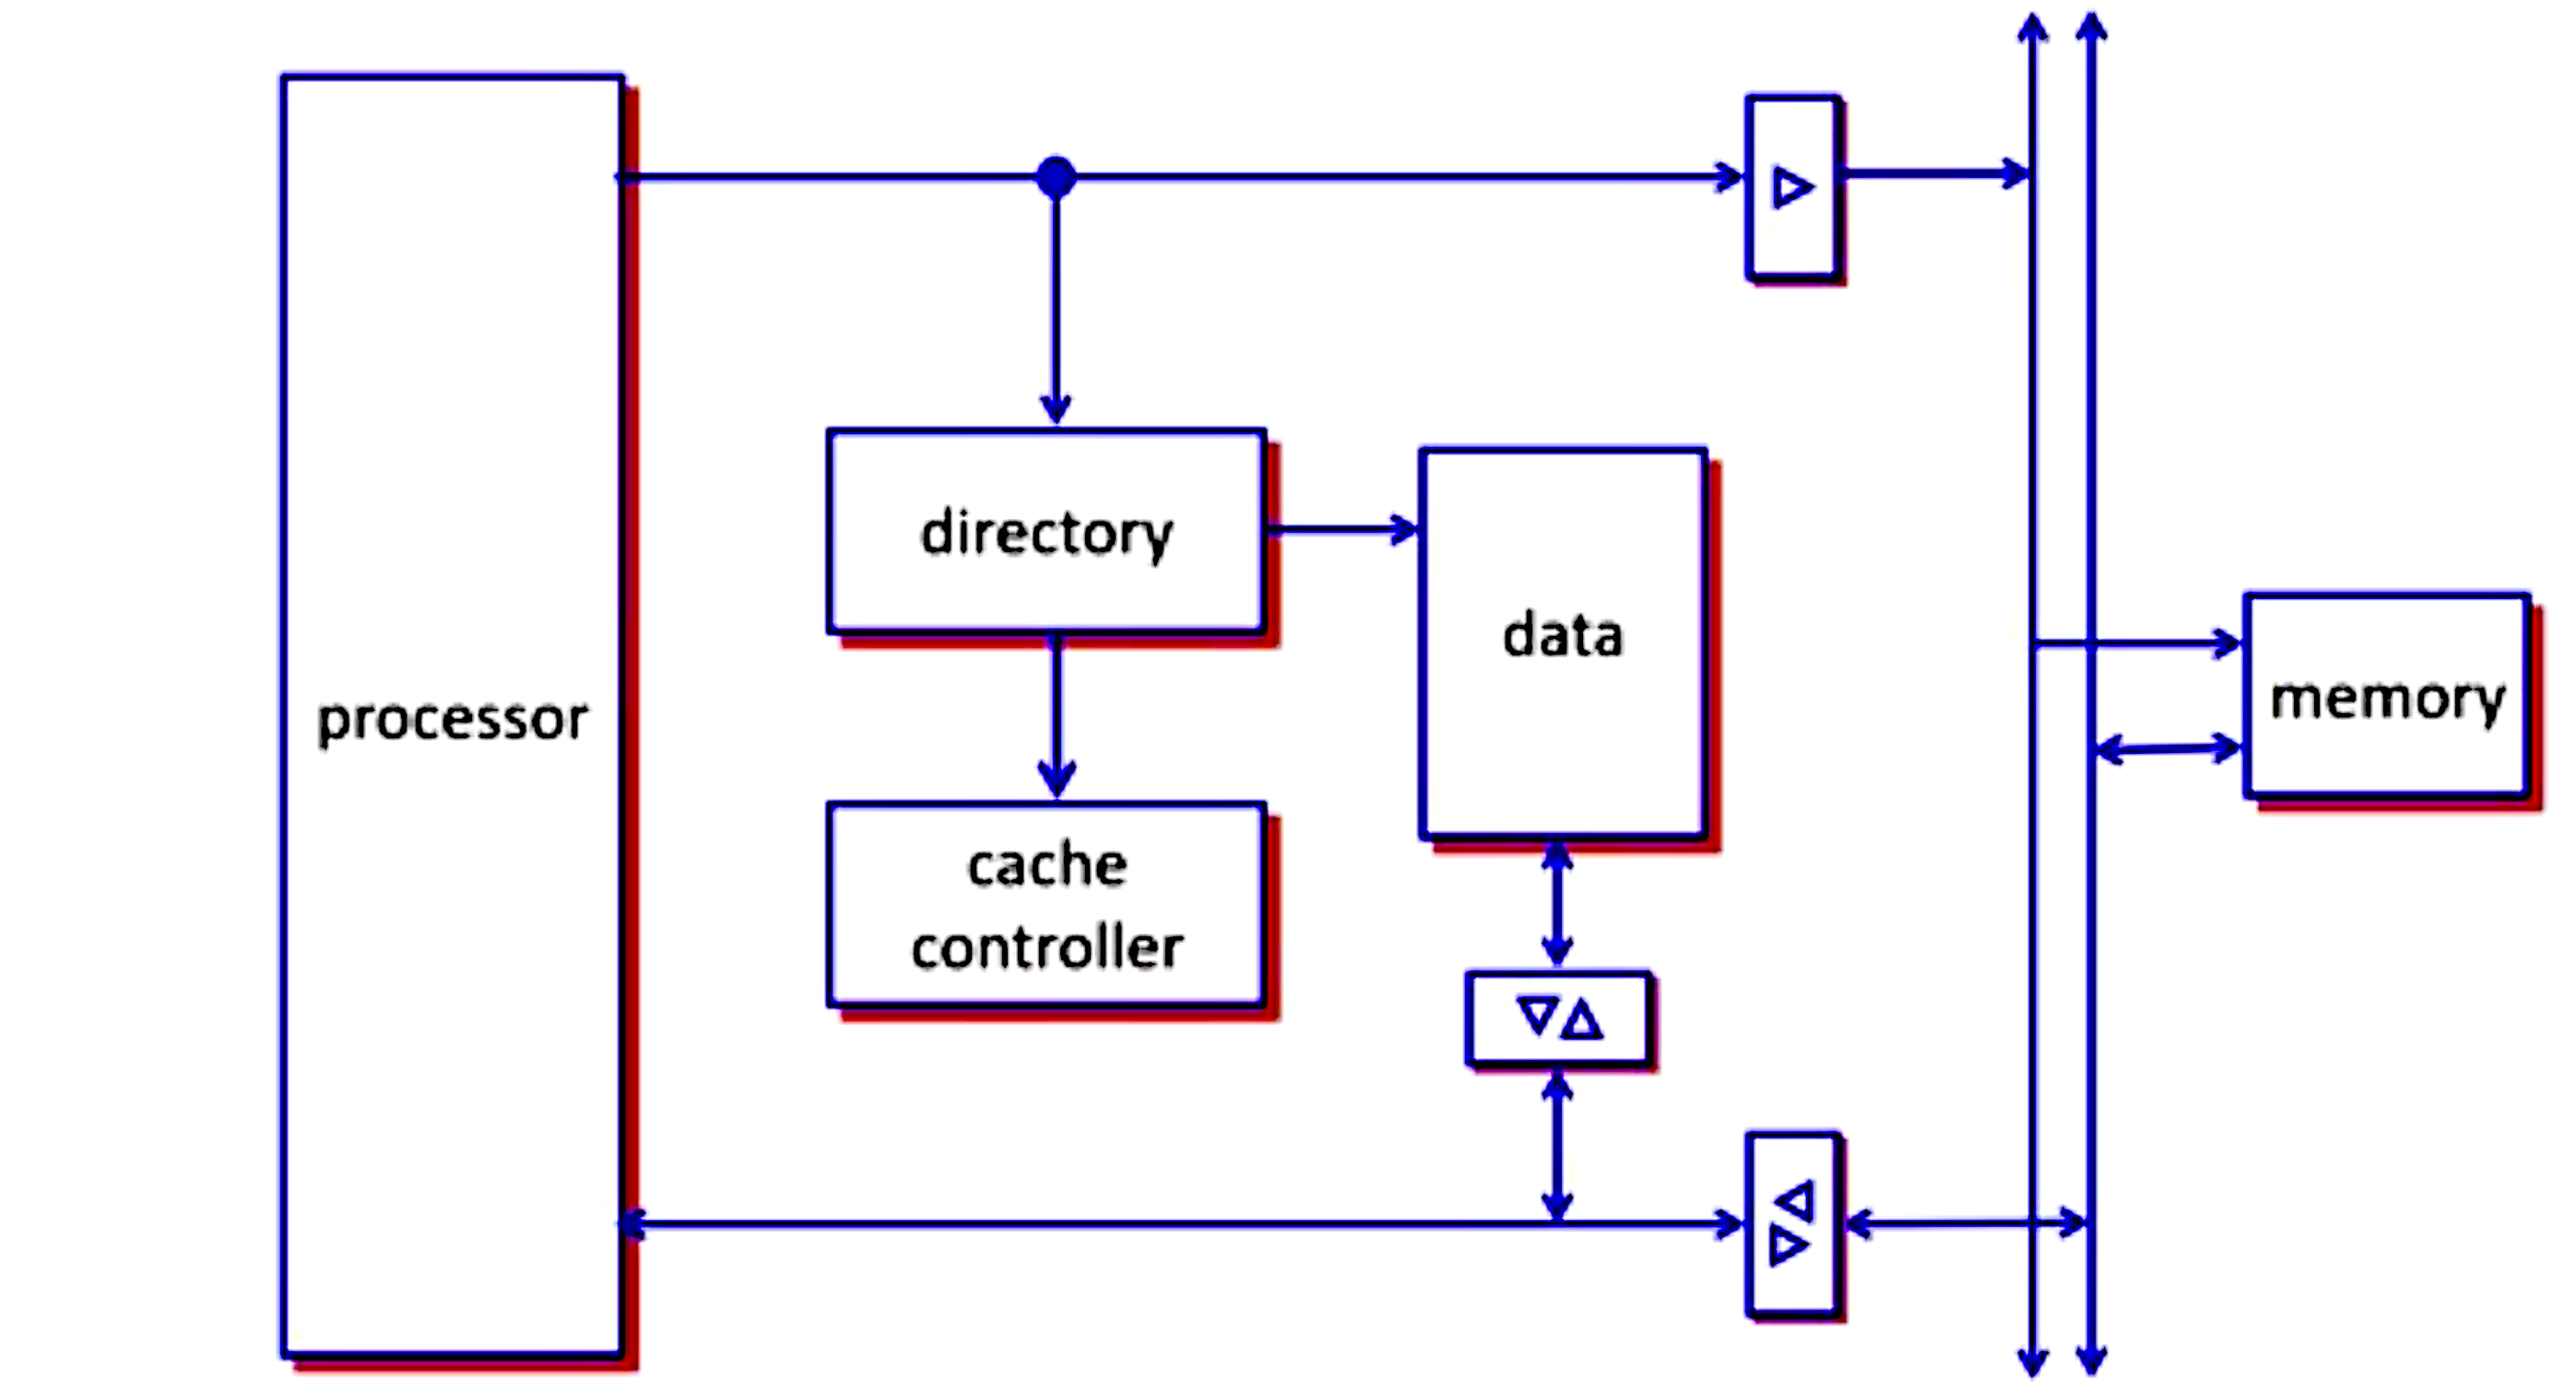
\includegraphics[width=0.55\textwidth]{chapters/chapter3a/images/cache_rep.png}
\end{center}

\begin{itemize}
    \item \textbf{Processor:} The central processing unit (CPU) that executes instructions and requests data from the memory hierarchy.

    \item \textbf{Directory:} A component that tracks the mapping of cached data to memory addresses. It determines whether a requested data item is present in the cache (cache hit) or not (cache miss).

    \item \textbf{Cache Controller:} This module manages the operation of the cache. It controls data flow between the directory, cache memory (data), and main memory. It ensures coherency and consistency of data when multiple memory requests occur.

    \item \textbf{Data:} The actual memory space within the cache that stores copies of frequently accessed data from main memory.

    \item \textbf{Main Memory:} The primary storage location that holds all data and instructions required by the processor. It communicates with the cache when the required data is not found in the cache (cache miss).

    \item \textbf{Bidirectional Arrows:} Indicate the flow of data between components. Data can flow from the processor to the cache, from the cache to the main memory, and vice versa.

    \item \textbf{Control Signals:} Represented as small triangular symbols, these signals are responsible for controlling the flow of data and ensuring synchronization between components.
\end{itemize}

\subsection{Cache Hit}
A \textit{cache hit} occurs when the processor requests data that is present in the cache. This scenario significantly improves performance by reducing the latency associated with memory access.
\begin{center}
    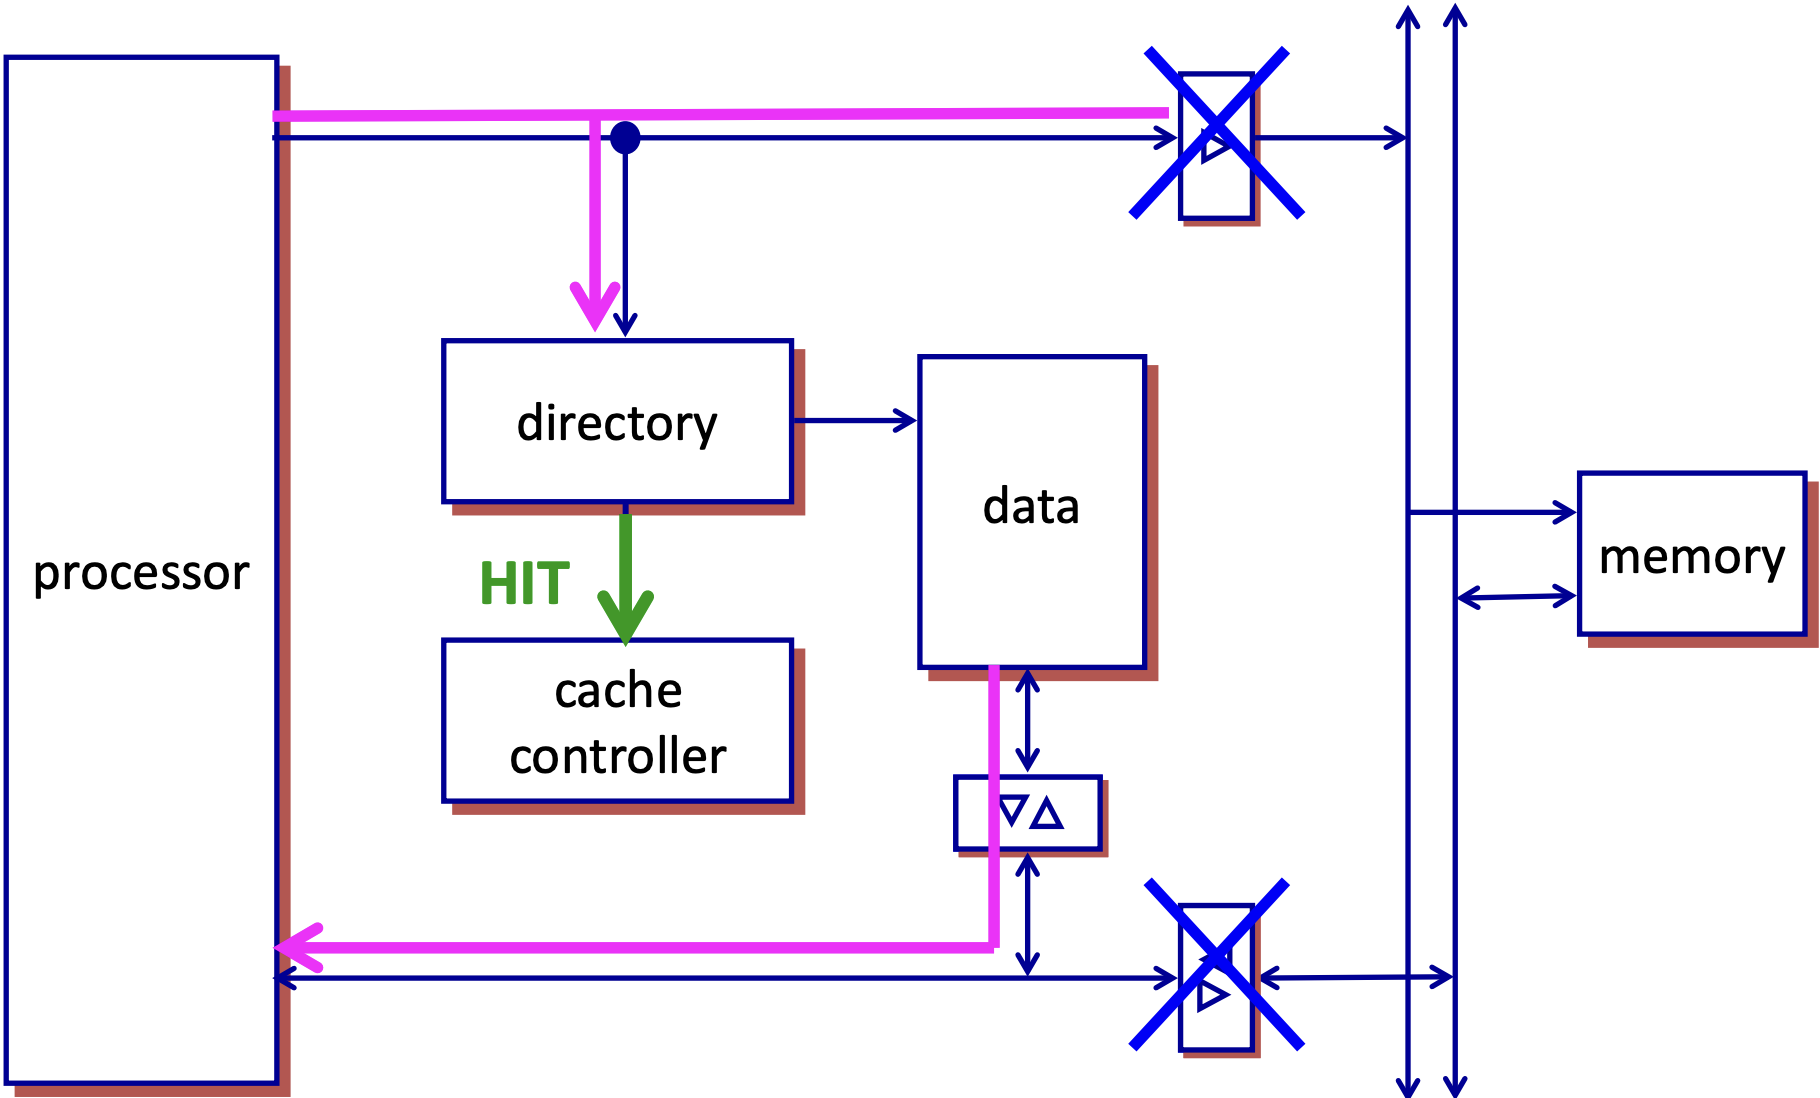
\includegraphics[width=0.55\textwidth]{chapters/chapter3a/images/hit.png}
\end{center}
\begin{enumerate}
    \item The processor sends a request for a specific data item.
    \item The \textit{directory} checks whether the requested data is available in the cache.
    \item If a match is found, a \textit{hit} is registered, and the \textit{cache controller} retrieves the data from the cache.
    \item The requested data is then sent directly back to the processor without accessing the main memory, as indicated by the absence of memory interaction in this scenario.
\end{enumerate}

\subsection{Cache Miss}
A cache miss occurs when the requested data is not present in the cache, requiring retrieval from the main memory. 
\begin{center}
    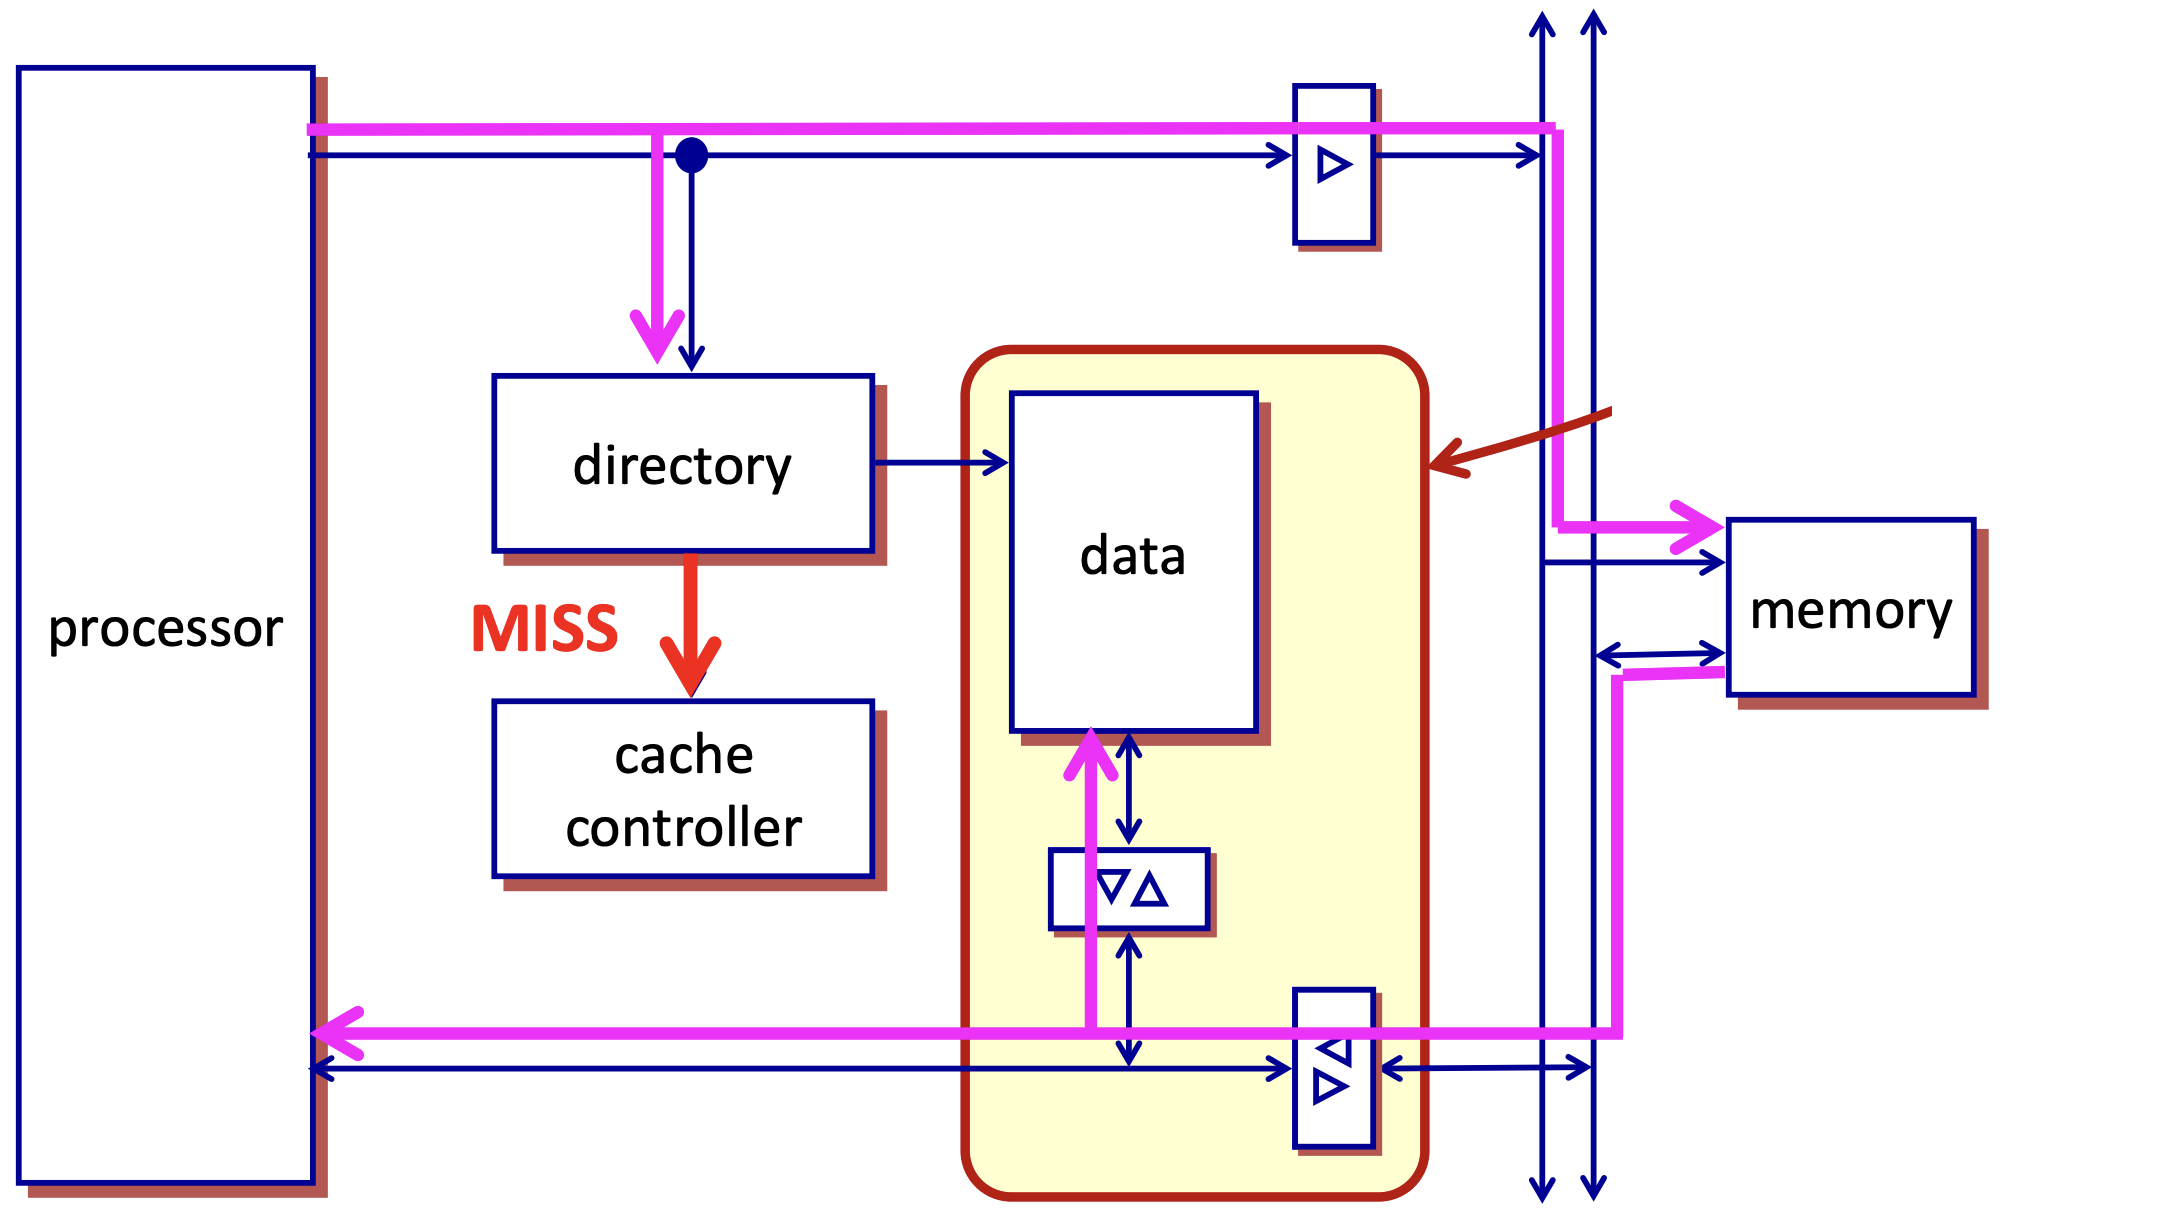
\includegraphics[width=0.55\textwidth]{chapters/chapter3a/images/miss.png}
\end{center}
\begin{enumerate}
    \item \textbf{Processor Request:} The processor issues a request for data. The request is forwarded to the cache directory.
    \item \textbf{Directory Check:} The directory checks whether the requested data is present in the cache. If the data is not found, a \textit{cache miss} is detected, and the directory informs the cache controller.
    \item \textbf{Cache Controller:} Upon detecting a cache miss, the cache controller initiates a fetch operation from the main memory. It ensures that the requested data is retrieved and forwarded to the processor.
    \item \textbf{Memory Access:} The cache controller sends a request to the main memory for the missing data. The memory responds by transferring the data back to the cache.
    \item \textbf{Cache Update:} The retrieved data is stored in the cache for future use. The directory is updated to reflect the new data location in the cache.
    \item \textbf{Processor Response:} Once the data is available in the cache, it is sent to the processor to fulfill the original request.
\end{enumerate}

\section{What if the Cache is Full?}
When the cache is full, adding new data requires the eviction of existing data to make space. This process is governed by a \textbf{cache replacement policy}. 
\begin{center}
    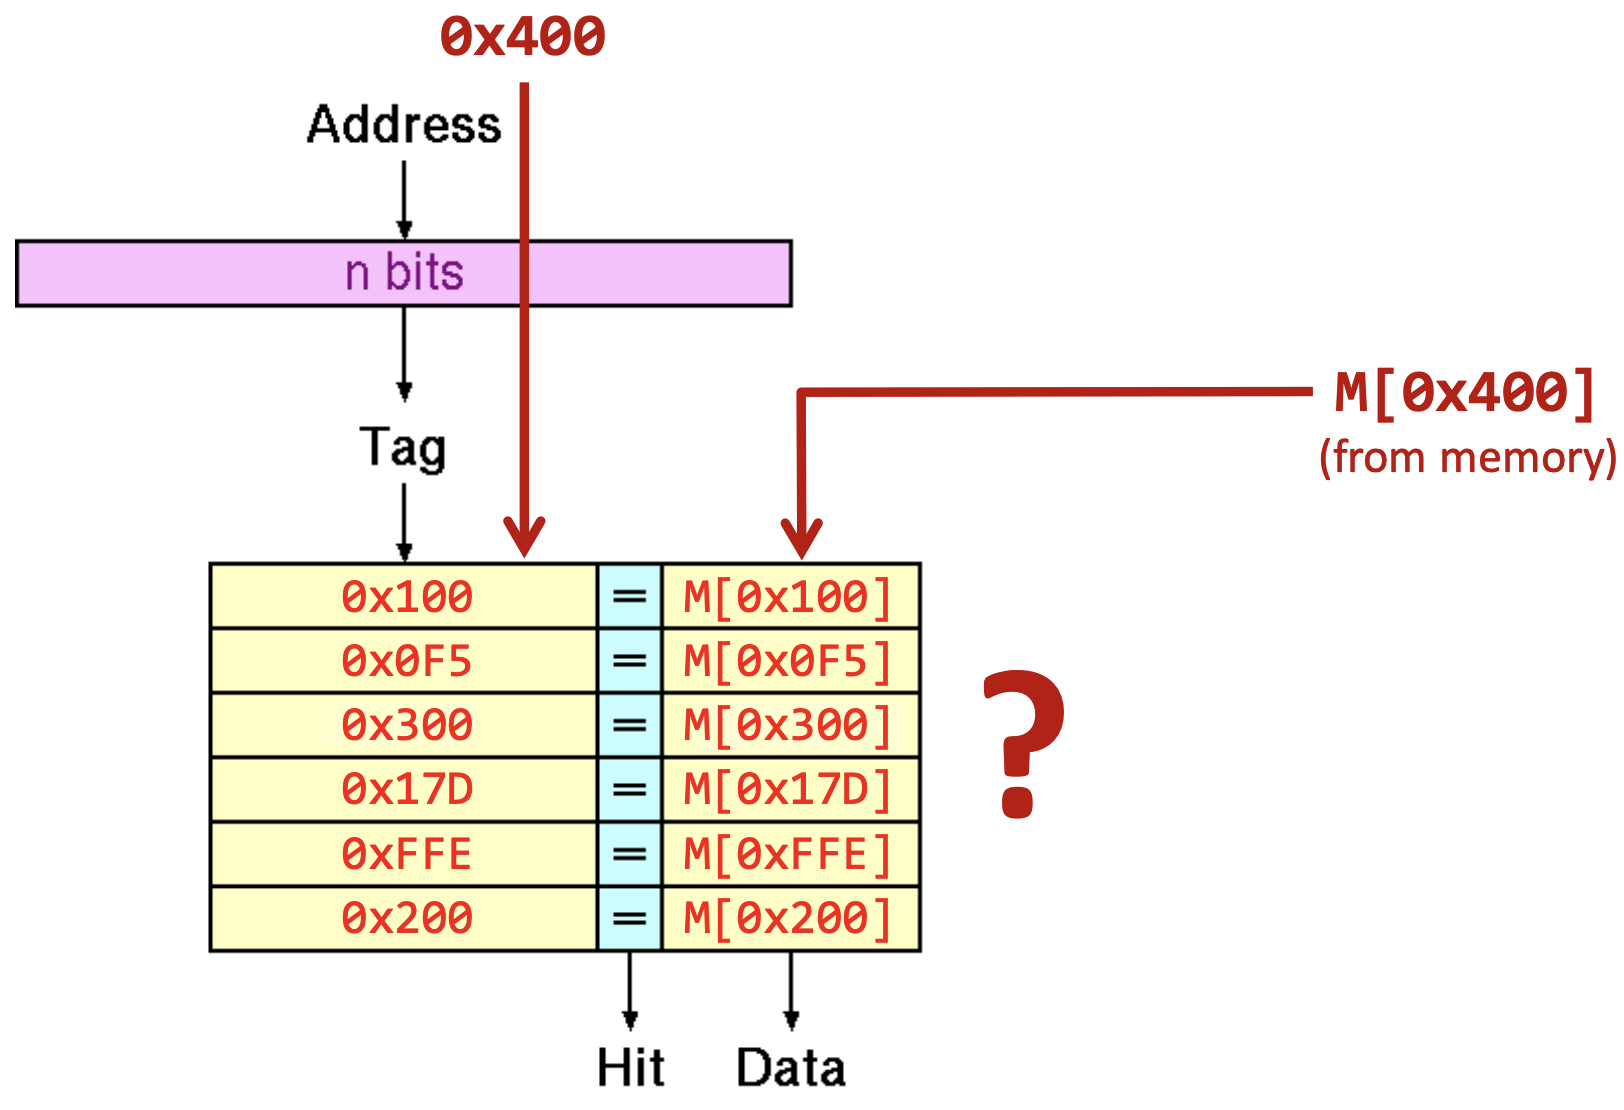
\includegraphics[width=0.65\textwidth]{chapters/chapter3a/images/full.png}
\end{center}
\subsection{Eviction Policies}
Various eviction policies determine which data to remove when the cache reaches its capacity limit. Common policies include:

    \item[-] \textbf{Least Recently Used (LRU):} 
    \begin{itemize}
        \item Replaces the data that has been unused for the longest time.
    \end{itemize}

    \item[-] \textbf{First-In-First-Out (FIFO):} 
    \begin{itemize}
        \item Evicts the oldest data in the cache, based on the order of entry.
    \end{itemize}

    \item[-] \textbf{Random Replacement:} 
    \begin{itemize}
        \item Selects a cache line at random for eviction, regardless of usage or age.
    \end{itemize}

    \item[-] \textbf{Approximate Schemes:} 
    \begin{itemize}
        \item Use heuristics or approximations to determine eviction, balancing simplicity and performance.
    \end{itemize}

Choosing the appropriate eviction policy depends on the application's requirements, balancing factors like speed, complexity, and data access patterns.

\subsection{Exploiting Temporal Locality}
Temporal locality refers to the principle that data recently accessed is likely to be accessed again in the near future. In this approach:

\begin{itemize}
    \item \textbf{Exclusive Data Fetching:} Only the specific data requested by the processor is fetched from the main memory into the cache, with the assumption that it will be reused soon.
    
    \item \textbf{Limitation:} This strategy does not account for \textit{spatial locality}, which predicts that data stored near the requested data is also likely to be accessed. For example:
    \begin{itemize}
        \item If the processor requests data at address \texttt{M[0x100]}, only this specific data is loaded into the cache.
        \item If the processor later requires data at \texttt{M[0x101]} (a neighboring address), it results in a cache miss since this data is not preloaded.
    \end{itemize}
    
    \item \textbf{Implication:} By focusing solely on temporal locality, the system may fail to optimize performance for workloads that benefit from spatial locality.
\end{itemize}

While exploiting temporal locality improves performance for certain types of workloads, balancing it with spatial locality considerations can further enhance efficiency.

\subsection{Only Exploiting Spatial Locality}
